
%%%%%%%%%%%%%%%%%%%%%%%%%%%%%%%%%%%%%%%%%%%%%%%%%%%%%%%%%%%%%%%%%%%%%%%%
\chapter{Introduction}
%%%%%%%%%%%%%%%%%%%%%%%%%%%%%%%%%%%%%%%%%%%%%%%%%%%%%%%%%%%%%%%%%%%%%%%%

\begin{center}
  \begin{minipage}{0.5\textwidth}
    \begin{small}
      Ice ice ice ice ice. I suppose this could be a quote about how ice has changed?
    \end{small}
  \end{minipage}
  \vspace{0.5cm}
\end{center}

\noindent This is an introduction to my thesis about ambient noise in the arctic

%%%%%%%%%%%%%%%%%%%%%%%%%%%%%%%%%%%%%%%%%%%%%%%%%%%%%%%%%%%%%%%%%%%%%%%%
\section{The Arctic Environment and the Beaufort Duct}
%%%%%%%%%%%%%%%%%%%%%%%%%%%%%%%%%%%%%%%%%%%%%%%%%%%%%%%%%%%%%%%%%%%%%%%%

\begin{enumerate}
\item Why do we care about the arctic and climate change?
anthropogenic factors:
biologic factors:
ecosystem?

\end{enumerate}



%%%%%%%%%%%%%%%%%%%%%%%%%%%%%%%%%%%%%%%%%%%%%%%%%%%%%%%%%%%%%%%%%%%%%%%%
\subsection{Noise in the Arctic}
%%%%%%%%%%%%%%%%%%%%%%%%%%%%%%%%%%%%%%%%%%%%%%%%%%%%%%%%%%%%%%%%%%%%%%%%
\begin{enumerate}
\item explain how sound travels underwater using an equation

\item explain how sound speed is affected by climate change
\end{enumerate}

figure from this rticle reproduced with concent from author (go get from jasa)
\begin{figure}[ht]
\centering
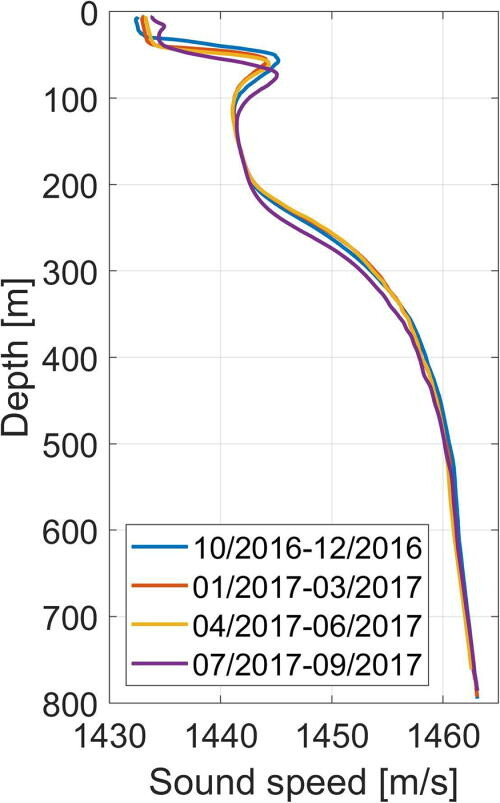
\includegraphics[scale=0.5]{Figures/ssp.jpeg}
\caption{Sound speed profiles in the Chukchi sea displaying presence of Beaufort duct. Image reproduced with author's permission}
\label{fig_ssp}
\end{figure}
%%%%%%%%%%%%%%%%%%%%%%%%%%%%%%%%%%%%%%%%%%%%%%%%%%%%%%%%%%%%%%
\section{The CANAPE Experiment}

what was this experiment?

where was this experiment?
we're SW-CANAPE, shallow water

why was this experiment performed?

when did it happen?

how did it happen? describe procedures
don't forget to ask julien for a canape figure about location/setup


%%%%%%%%%%%%%%%%%%%%%%%%%%%%%%%%%%%%%%%%%%%%%%%%%%%%%%%%%%%%%%
\subsection{Data Collection}

how was data collected

what was the form of the data

how was it processed?
% 'spectral analysis of acoustic data section
The acoustic data collected by the SHRUs was processed using...
\footcite[]{Bonnel2021}

%%%%%%%%%%%%%%%%%%%%%%%%%%%%%%%%%%%%%%%%%%%%%%%%%%%%%%%%%%%%%%%%%%%
\subsection{Environmental Data} \label{env_info}
am i allowed to use the ssp in original paper?


how are the different acoustic environments defined.

where did the data come from?

how was the data processed?

ABSOLUTELY MAKE SURE TO DEFINE what each condition means and when it happened so we get the approximate time length
'ice with duct' occurs when there is ice present and it 
'ice without duct' occurs when there is ice present but the Beaufort duct does not exist. The approximate time period covered  are during [] to [].                                                                                            
'no ice' occurs when there is no ice or less than [certain amount] of ice. This environmental time period covers...
The environmental condition of 'no ice' also means that there is no duct.
%%%%%%%%%%%%%%%%%%%%%%%%%%%%%%%%%%%%%%%%%%%%%%%%%%%%%%%%%%%%%%%
% end of introduction